% =====================================================================
% 5. Area 3: generative AI, autoregressive generators of the ECG (T23, own block)
% =====================================================================
\section{Area 3: autoregressive generation of the ECG (own block)}\label{sec:generative}

\subsection{Theory: autoregressive models}

An autoregressive model writes the probability of a sequence as a product of conditionals,
\begin{equation}
p(u_1,\dots,u_T) = \prod_{t=1}^{T} p(u_t \mid u_1,\dots,u_{t-1}),
\end{equation}
and learns the conditional of the next symbol. GPT-style language models are trained with ``a standard
language modeling objective'', the sum of $\log P(u_i \mid u_{i-k},\dots,u_{i-1})$ over a context of $k$
symbols \cite[p.~3]{radford2018improving}, using ``a 12-layer decoder-only transformer with masked
self-attention heads'' \cite[p.~5]{radford2018improving}. Two ideas make training efficient.
\emph{Teacher forcing}: the input is the true sequence and the target is the same sequence shifted by
one, so every position of a window is a training example. The \emph{causal mask}: the attention score of
every future position is set to $-\infty$ before the softmax, so position $t$ sees only $u_1,\dots,u_t$
and the whole window is processed in one parallel pass without the model reading its own target. The
loss is the cross-entropy between the predicted distribution and the observed next symbol, the usual
loss of a language model \cite[p.~3]{chelba2017ngram}; perplexity, its exponential, is the classical
quality measure of a language model \cite[p.~2]{chelba2017ngram}. Generation then samples one symbol at
a time and feeds it back as input.

The cross-entropy per token depends on the vocabulary: coarse tokens are easier to guess. To compare
vocabularies we report \emph{bits per sample}, the cost of coding the microvolt value of the next
sample:
\begin{equation}
\text{bits per sample} = \frac{\mathrm{CE} + \ln \Delta}{\ln 2},
\end{equation}
where CE is the cross-entropy in nats and $\Delta$ the number of microvolt values in one token,
assuming they are equally likely inside the token. Reporting entropy in bits per symbol has a
precedent in character-level models \cite[p.~8]{pascanu2013difficulty}; that it makes vocabularies
comparable is our own argument (with $\Delta = 1$ it is the cross-entropy in bits).

\subsection{Design}

\paragraph{Tokens.} PTB-XL stores every sample as an integer number of microvolts, so lead II becomes a
sequence of symbols without loss of information: each sample is mapped to one of $V$ levels of $\Delta$
microvolts over a range of 2.56\,mV taken from the training data, values outside going to the first or
last token. The baseline uses $V = 256$ ($\Delta = 10$\,\textmu V, an error far below the signal's
spread), with $V = 64$ and $V = 2560$ (one token per microvolt) as ablations. Turning amplitudes into
discrete symbols is also the approach of recent ECG language models, which ``use quantization to
represent amplitude ranges as discrete symbols'' \cite[p.~2]{han2025ecgbyte}. Non-uniform (mu-law)
quantisation was not tried.

\paragraph{Models and training.} The \emph{ECG-GPT} is a decoder-only Transformer: a learned embedding
per token, sinusoidal positional encoding of the position in the window, two Pre-LN blocks with causal
self-attention (four heads; the blocks of Mar\'ia's Transformer with the mask switched on), a final
LayerNorm and a Linear layer to $V$ logits (\generativeParamsBase{} parameters). The comparison model is
a two-layer \emph{LSTM} of the same size (\generativeParamsLstm{} parameters), causal by construction.
Both read windows of $L = 250$ samples (2.5\,s) drawn at random positions of the training records of
folds 1--8 (also those without a superclass; no label is used) and are evaluated on fixed windows that
cover every sample of the validation records. The test fold is never read. Training followed the shared
protocol with a 50-epoch budget and three seeds per configuration. Ablations: LSTM, context of 1\,s and
5\,s, $V = 64$ and 2560, no positional encoding, and no causal mask (to show why it is needed).

\subsection{Results}

% Shared float (common/make_floats.py). Table: tables/generative_ablations.tex
\begin{table}[htbp]
\centering
\caption[Generators: ablations (validation)]{Generators of lead II on the validation fold (mean $\pm$ SD over seeds 42--44). CE: cross-entropy per token (nats), not comparable across vocabularies; bits per sample: comparable; $\Delta$ bits: mean paired difference with the baseline (negative = better). The model without the causal mask is not compared (it sees its target).}
\label{tab:generative_ablations}
\small
\begin{adjustbox}{max width=\textwidth}
% Generated by src/generative_experiments.py from results/logs/generative_summary.json.
% Needs report/numbers.tex (alias "generative" in report/runs.json) and \usepackage{booktabs}. Wide: use \resizebox{\textwidth}{!}{...}.
% CE: validation cross-entropy per token (nats); it depends on the vocabulary. Bits: bits per sample, comparable across vocabularies.
% Delta: paired difference in bits with the baseline, same seed; negative = fewer bits. Last: CE at the last position of the window.
\begin{tabular}{llrrrccccr}
\toprule
Factor & Configuration & Parameters & $L$ & $V$ & CE (nats) & Bits per sample & $\Delta$ bits & Seeds better / worse & Last-position CE \\
\midrule
baseline & ECG-GPT: causal Transformer, 2 blocks, $L$ = 250, $V$ = 256 & \generativeParamsBase{} & \generativeContextBase{} & \generativeVocabBase{} & \generativeCeMeanBase{} $\pm$ \generativeCeSdBase{} & \generativeBitsMeanBase{} $\pm$ \generativeBitsSdBase{} & --- & --- & \generativeCeLastMeanBase{} \\
\addlinespace
architecture & LSTM, 2 layers of 160 (same size) & \generativeParamsLstm{} & \generativeContextLstm{} & \generativeVocabLstm{} & \generativeCeMeanLstm{} $\pm$ \generativeCeSdLstm{} & \generativeBitsMeanLstm{} $\pm$ \generativeBitsSdLstm{} & \generativeDiffMeanLstm{} & \generativeNSeedsBetterLstm{} / \generativeNSeedsWorseLstm{} of \generativeNSeedsComparedLstm{} & \generativeCeLastMeanLstm{} \\
\addlinespace
context length & Context of 100 samples (1 s) & \generativeParamsCtxOneZeroZero{} & \generativeContextCtxOneZeroZero{} & \generativeVocabCtxOneZeroZero{} & \generativeCeMeanCtxOneZeroZero{} $\pm$ \generativeCeSdCtxOneZeroZero{} & \generativeBitsMeanCtxOneZeroZero{} $\pm$ \generativeBitsSdCtxOneZeroZero{} & \generativeDiffMeanCtxOneZeroZero{} & \generativeNSeedsBetterCtxOneZeroZero{} / \generativeNSeedsWorseCtxOneZeroZero{} of \generativeNSeedsComparedCtxOneZeroZero{} & \generativeCeLastMeanCtxOneZeroZero{} \\
\addlinespace
vocabulary & 64 levels of 40 $\mu$V & \generativeParamsVocabSixFour{} & \generativeContextVocabSixFour{} & \generativeVocabVocabSixFour{} & \generativeCeMeanVocabSixFour{} $\pm$ \generativeCeSdVocabSixFour{} & \generativeBitsMeanVocabSixFour{} $\pm$ \generativeBitsSdVocabSixFour{} & \generativeDiffMeanVocabSixFour{} & \generativeNSeedsBetterVocabSixFour{} / \generativeNSeedsWorseVocabSixFour{} of \generativeNSeedsComparedVocabSixFour{} & \generativeCeLastMeanVocabSixFour{} \\
\addlinespace
positional encoding & No positional encoding & \generativeParamsNoPos{} & \generativeContextNoPos{} & \generativeVocabNoPos{} & \generativeCeMeanNoPos{} $\pm$ \generativeCeSdNoPos{} & \generativeBitsMeanNoPos{} $\pm$ \generativeBitsSdNoPos{} & \generativeDiffMeanNoPos{} & \generativeNSeedsBetterNoPos{} / \generativeNSeedsWorseNoPos{} of \generativeNSeedsComparedNoPos{} & \generativeCeLastMeanNoPos{} \\
\addlinespace
causal mask & No causal mask (sees the future) & \generativeParamsNoMask{} & \generativeContextNoMask{} & \generativeVocabNoMask{} & \generativeCeMeanNoMask{} $\pm$ \generativeCeSdNoMask{} & \generativeBitsMeanNoMask{} $\pm$ \generativeBitsSdNoMask{} & --- & --- & \generativeCeLastMeanNoMask{} \\
\addlinespace
vocabulary & 2560 levels of 1 $\mu$V (lossless) & \generativeParamsVocabTwoFiveSixZero{} & \generativeContextVocabTwoFiveSixZero{} & \generativeVocabVocabTwoFiveSixZero{} & \generativeCeMeanVocabTwoFiveSixZero{} $\pm$ \generativeCeSdVocabTwoFiveSixZero{} & \generativeBitsMeanVocabTwoFiveSixZero{} $\pm$ \generativeBitsSdVocabTwoFiveSixZero{} & \generativeDiffMeanVocabTwoFiveSixZero{} & \generativeNSeedsBetterVocabTwoFiveSixZero{} / \generativeNSeedsWorseVocabTwoFiveSixZero{} of \generativeNSeedsComparedVocabTwoFiveSixZero{} & \generativeCeLastMeanVocabTwoFiveSixZero{} \\
\addlinespace
context length & Context of 500 samples (5 s) & \generativeParamsCtxFiveZeroZero{} & \generativeContextCtxFiveZeroZero{} & \generativeVocabCtxFiveZeroZero{} & \generativeCeMeanCtxFiveZeroZero{} $\pm$ \generativeCeSdCtxFiveZeroZero{} & \generativeBitsMeanCtxFiveZeroZero{} $\pm$ \generativeBitsSdCtxFiveZeroZero{} & \generativeDiffMeanCtxFiveZeroZero{} & \generativeNSeedsBetterCtxFiveZeroZero{} / \generativeNSeedsWorseCtxFiveZeroZero{} of \generativeNSeedsComparedCtxFiveZeroZero{} & \generativeCeLastMeanCtxFiveZeroZero{} \\
\midrule
\multicolumn{10}{l}{\emph{Baselines without training (bits per sample on the same validation records)}} \\
\multicolumn{6}{l}{Uniform over the range} & \generativeUniformBits{} & & & \\
\multicolumn{6}{l}{Unigram / bigram counts, $V$ = 64} & \generativeUnigramBitsVSixFour{} / \generativeBigramBitsVSixFour{} & & & \\
\multicolumn{6}{l}{Unigram / bigram counts, $V$ = 256} & \generativeUnigramBitsVTwoFiveSix{} / \generativeBigramBitsVTwoFiveSix{} & & & \\
\multicolumn{6}{l}{Unigram / bigram counts, $V$ = 2560} & \generativeUnigramBitsVTwoFiveSixZero{} / \generativeBigramBitsVTwoFiveSixZero{} & & & \\
\bottomrule
\end{tabular}

\end{adjustbox}
\end{table}


\begin{enumerate}[leftmargin=1.4em,itemsep=2pt]
  \item \textbf{The models learn far more than local smoothness.} The ECG-GPT baseline codes the next
        sample with \generativeBitsMeanBase{} bits, against \generativeBigramBitsVTwoFiveSix{} for a bigram
        model obtained by counting token pairs and \generativeUniformBits{} for uniform guessing; its
        prediction error (\generativeRmseUvMeanBase{}\,\textmu V) is well below that of ``next sample =
        this sample'' (\generativePersistenceRmseUv{}\,\textmu V). Every configuration with the causal
        mask beats the bigram model of its own vocabulary.
  \item \textbf{Bits, not cross-entropy, rank the vocabularies.} Cross-entropy alone would rank $V = 64$
        first (\generativeCeMeanVocabSixFour{} nats) and $V = 2560$ last (\generativeCeMeanVocabTwoFiveSixZero{});
        in bits the order is reversed: one-microvolt tokens are the best of the grid
        (\generativeDiffMeanVocabTwoFiveSixZero{} against the baseline) and 40\,\textmu V tokens the worst
        (\generativeDiffMeanVocabSixFour{}). With coarse tokens the uniform-within-token assumption
        wastes bits, because on flat segments the next sample is usually within a few microvolts of the
        current one.
  \item \textbf{Context and the previous beat.} A context of 1\,s is worse in every seed
        (\generativeDiffMeanCtxOneZeroZero{}) and 5\,s better (\generativeDiffMeanCtxFiveZeroZero{}).
        The cost per position (Figure~\ref{fig:generative_context}) falls with the context available and
        drops a second time at about one second, roughly one heartbeat. \emph{Hypothesis:} once a whole
        previous beat is in the window, the model can anticipate the next QRS. The comparison is at equal
        epochs, so the 5\,s model saw twice as many samples.
  \item \textbf{Positional encoding matters when generating.} Without it the ECG-GPT is clearly worse
        (\generativeDiffMeanNoPos{}, every seed) and its cost curve shows no drop at one beat. This is the
        opposite of the classifier, which did better without positions (Section~\ref{sec:transformer}).
        The literature reports that language models ``without any explicit positional encoding are still
        competitive'' \cite[p.~1]{haviv2022transformer}; our setting differs (short windows of a periodic
        signal, a small model and a fixed budget), and the explanation of our result is a hypothesis:
        to use the previous beat, the model needs to know how far back it was.
  \item \textbf{LSTM against causal Transformer.} At equal size, data and budget the LSTM codes the
        signal with fewer bits (\generativeDiffMeanLstm{}, every seed). Why is not established: the
        recurrence may suit a smooth, locally predictable signal, and our Transformer has two blocks only.
  \item \textbf{Without the causal mask the model reads the answer.} Its teacher-forced cross-entropy
        falls to \generativeCeMeanNoMask{} nats within a few epochs (Figure~\ref{fig:generative_curves}c),
        but at the last position of the window, the only one whose target is not in the input, it is
        worse than the baseline (\generativeCeLastMeanNoMask{} against \generativeCeLastMeanBase{} nats),
        and its samples are the worst of the grid. The mask is what makes parallel teacher-forced training
        honest.
\end{enumerate}

% Shared float (common/make_floats.py). Figure: figures/generative_context.pdf
\begin{figure}[htbp]
\centering
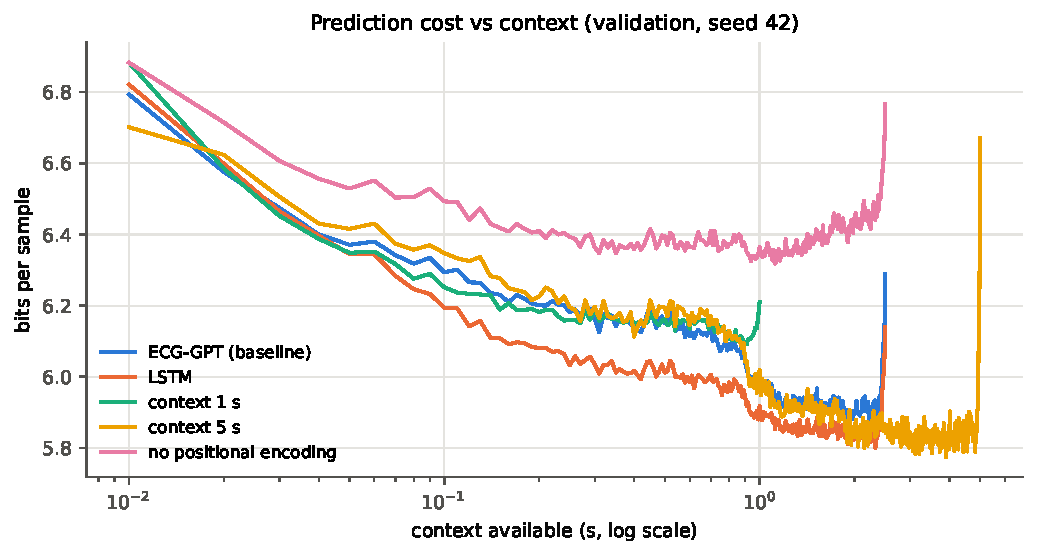
\includegraphics[width=\textwidth,height=0.42\textheight,keepaspectratio]{figures/generative_context.pdf}
\caption[Generators: prediction cost against context]{Prediction cost against the context available (validation, seed 42): bits per sample at each position of the window, i.e.\ predicting with $t+1$ past samples. Logarithmic horizontal axis.}
\label{fig:generative_context}
\end{figure}

% Shared float (common/make_floats.py). Figure: figures/generative_curves.pdf
\begin{figure}[htbp]
\centering
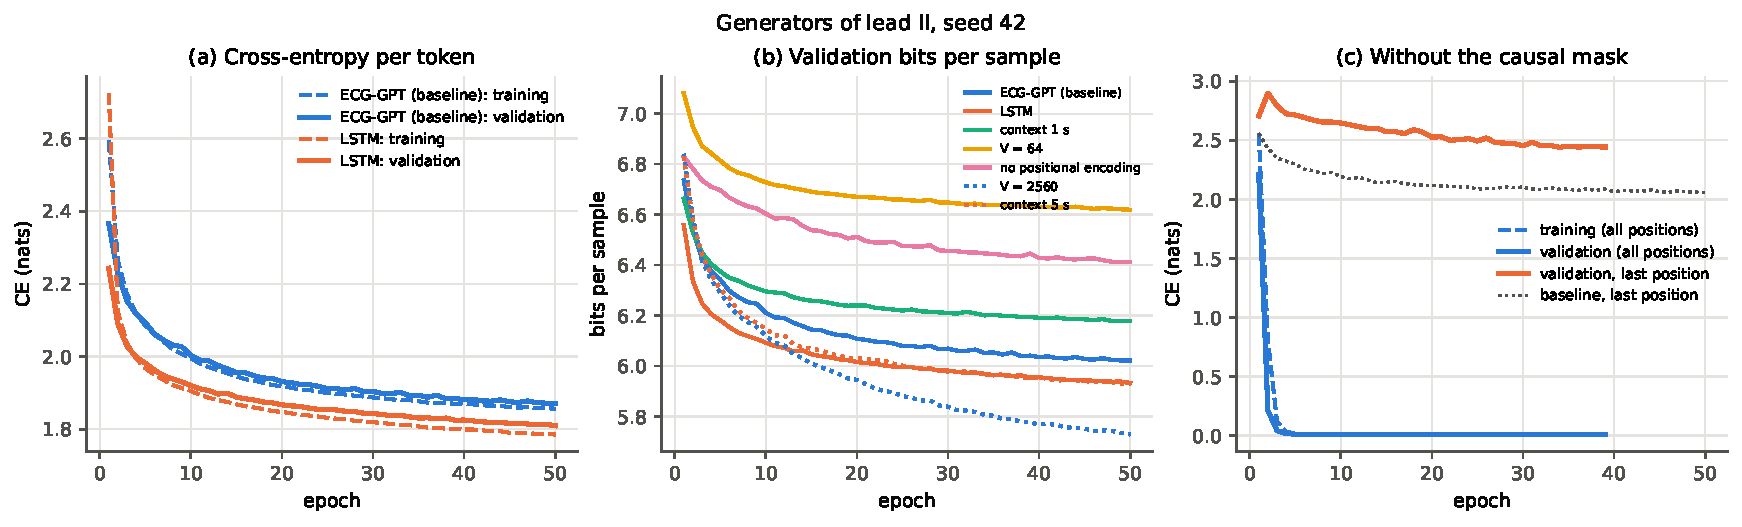
\includegraphics[width=\textwidth,height=0.42\textheight,keepaspectratio]{figures/generative_curves.pdf}
\caption[Generators: learning curves]{Generators of lead II, seed 42. (a) Cross-entropy per token of the ECG-GPT baseline and the LSTM. (b) Validation bits per sample of every configuration. (c) The ECG-GPT without the causal mask: training and validation cross-entropy over all positions and at the last position, with the baseline's last position for reference.}
\label{fig:generative_curves}
\end{figure}


\paragraph{Training budget.} Almost every run reached the 50-epoch limit with its best epoch at or near
the end: no generator had fully converged. The last epochs changed the bits by much less than the
differences reported, so the comparisons stand as comparisons at equal budget, not between converged
models.

\subsection{Generation and sampling}

Each generator received the first 2\,s of 256 validation records as a prompt and generated the next
8\,s, sliding its window one sample at a time, as in the course notebooks \cite{course_nb_sampling}.
We compared \emph{greedy search} (always the most probable token), sampling with a \emph{temperature}
$T$ (logits divided by $T$ before the softmax: low $T$ sharpens the distribution, high $T$ flattens it)
and \emph{top-$k$} sampling, introduced by Fan et al., who ``randomly sample from the $k = 10$ most
likely candidates'' \cite[p.~893]{fan2018hierarchical}. Nucleus sampling, which keeps ``the highest
probability tokens whose cumulative probability mass exceeds the pre-chosen threshold $p$''
\cite[p.~5]{holtzman2020curious}, was not needed for the comparison and was not run.

% Shared float (common/make_floats.py). Figure: figures/generative_samples.pdf
\begin{figure}[htbp]
\centering
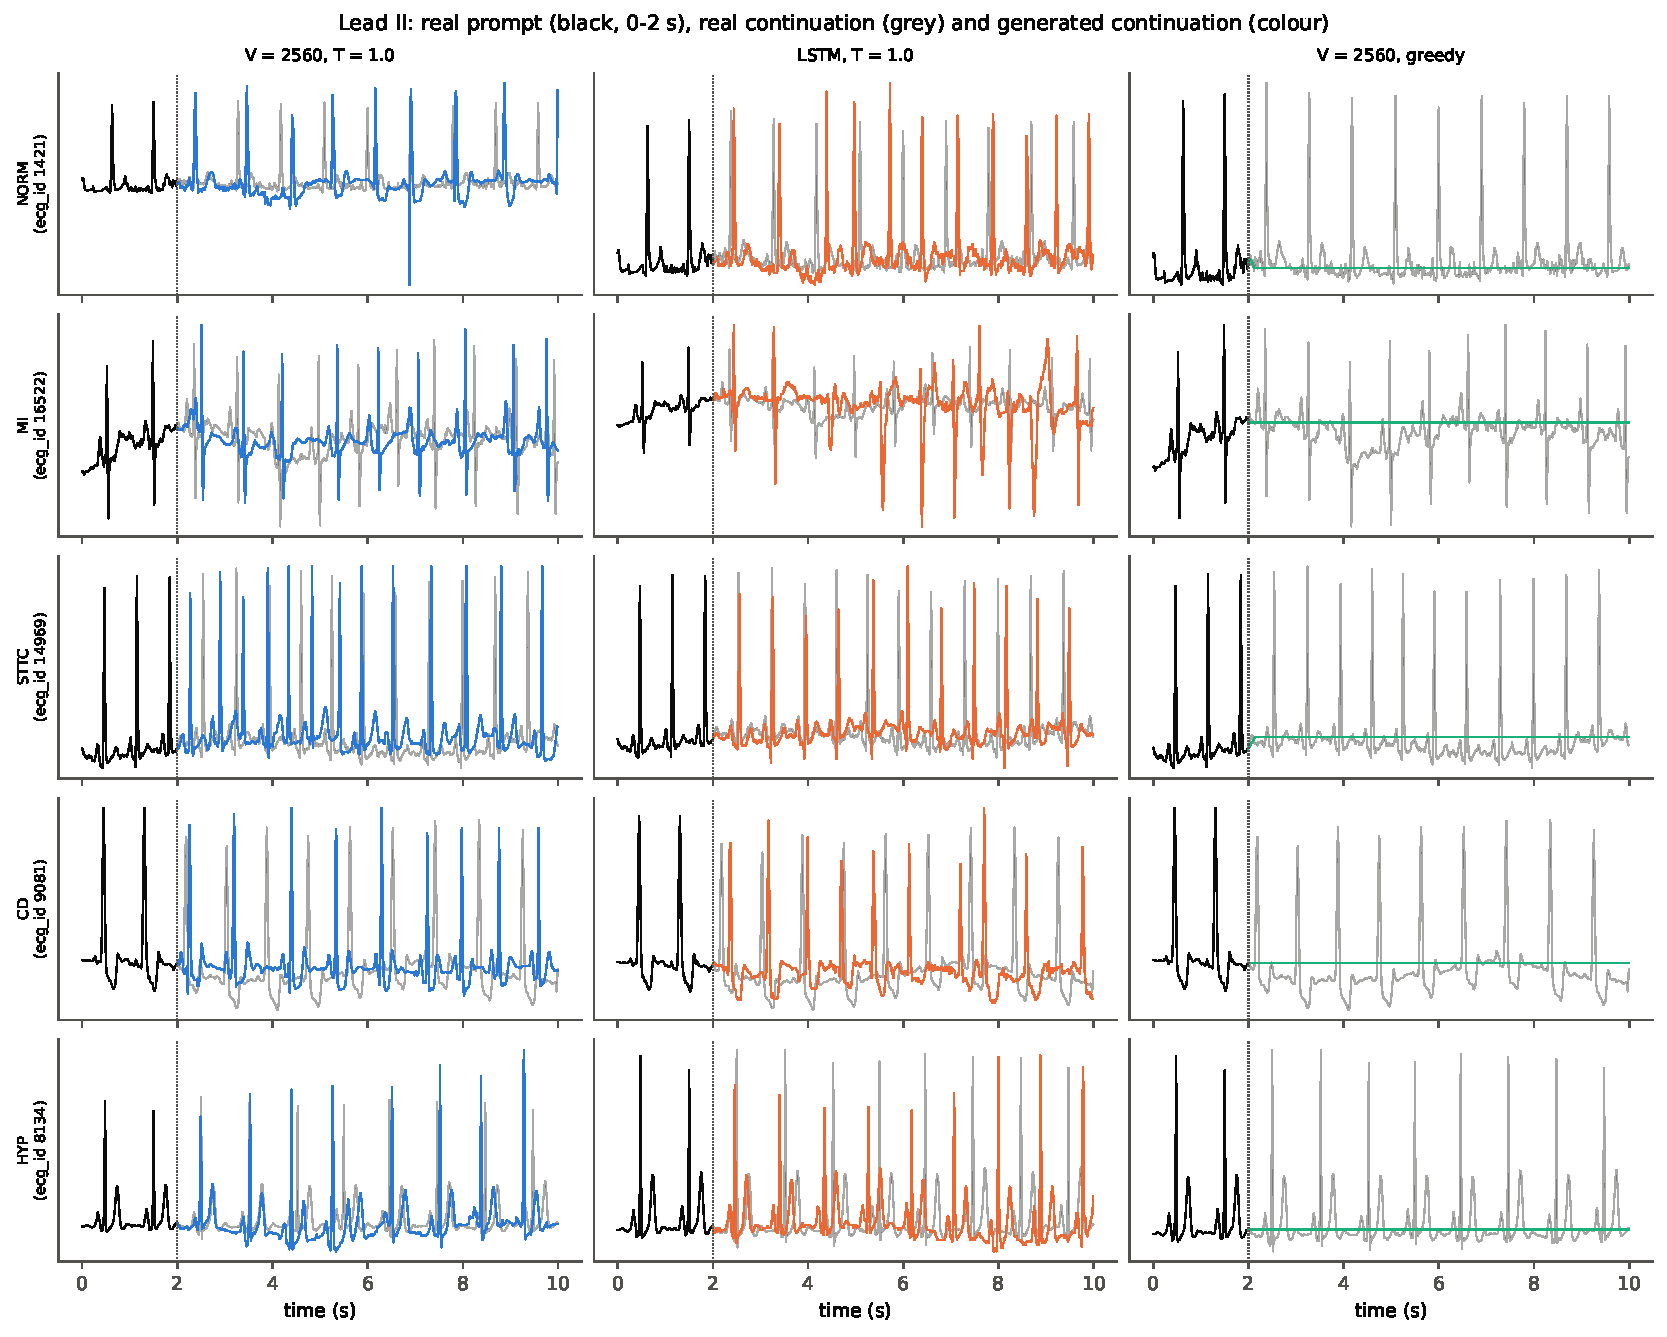
\includegraphics[width=\textwidth,height=0.42\textheight,keepaspectratio]{figures/generative_samples.pdf}
\caption[Generators: real and generated lead II]{Lead II of one validation record per superclass: real 2\,s prompt (black), real continuation (grey) and generated continuation (colour) of the selected ECG-GPT ($V = 2560$, $T = 1$), the LSTM ($T = 1$) and the ECG-GPT with greedy search.}
\label{fig:generative_samples}
\end{figure}

% Shared float (common/make_floats.py). Table: tables/generative_sampling.tex
\begin{table}[htbp]
\centering
\caption[Generators: generation statistics]{Generation statistics (seed-42 models, 256 validation records, 2\,s prompt, 8\,s generated): median ratio of generated to real standard deviation; share of flat records; Wasserstein-1 distance between amplitude distributions; share of records with a detected heart rate and mean absolute heart-rate error.}
\label{tab:generative_sampling}
\small
\begin{adjustbox}{max width=\textwidth}
% Generated by src/generative_experiments.py from results/logs/generative_summary.json.
% 2 s of real lead II as prompt, 8 s generated, compared with the real 8 s of the same validation records (seed-42 models).
% Std ratio: median std(generated) / std(real). Flat: share of records whose last 4 s are almost constant.
% W1: Wasserstein distance between amplitude distributions (mV). HR: heart rate from R peaks (simple threshold rule).
\begin{tabular}{llccccc}
\toprule
Model & Sampling & Std ratio & Flat & W1 (mV) & HR found & HR error (bpm) \\
\midrule
$V$ = 2560 & greedy & \generativeGenVocabTwoFiveSixZeroGreedyStdRatio{} & \generativeGenVocabTwoFiveSixZeroGreedyFracFlat{} & \generativeGenVocabTwoFiveSixZeroGreedyWOneMv{} & \generativeGenVocabTwoFiveSixZeroGreedyHrDefinedFrac{} & --- \\
$V$ = 2560 & $T = 0.5$ & \generativeGenVocabTwoFiveSixZeroTZeroFiveStdRatio{} & \generativeGenVocabTwoFiveSixZeroTZeroFiveFracFlat{} & \generativeGenVocabTwoFiveSixZeroTZeroFiveWOneMv{} & \generativeGenVocabTwoFiveSixZeroTZeroFiveHrDefinedFrac{} & \generativeGenVocabTwoFiveSixZeroTZeroFiveHrMae{} \\
$V$ = 2560 & $T = 0.8$ & \generativeGenVocabTwoFiveSixZeroTZeroEightStdRatio{} & \generativeGenVocabTwoFiveSixZeroTZeroEightFracFlat{} & \generativeGenVocabTwoFiveSixZeroTZeroEightWOneMv{} & \generativeGenVocabTwoFiveSixZeroTZeroEightHrDefinedFrac{} & \generativeGenVocabTwoFiveSixZeroTZeroEightHrMae{} \\
$V$ = 2560 & $T = 1.0$ & \generativeGenVocabTwoFiveSixZeroTOneZeroStdRatio{} & \generativeGenVocabTwoFiveSixZeroTOneZeroFracFlat{} & \generativeGenVocabTwoFiveSixZeroTOneZeroWOneMv{} & \generativeGenVocabTwoFiveSixZeroTOneZeroHrDefinedFrac{} & \generativeGenVocabTwoFiveSixZeroTOneZeroHrMae{} \\
$V$ = 2560 & $T = 1.5$ & \generativeGenVocabTwoFiveSixZeroTOneFiveStdRatio{} & \generativeGenVocabTwoFiveSixZeroTOneFiveFracFlat{} & \generativeGenVocabTwoFiveSixZeroTOneFiveWOneMv{} & \generativeGenVocabTwoFiveSixZeroTOneFiveHrDefinedFrac{} & \generativeGenVocabTwoFiveSixZeroTOneFiveHrMae{} \\
$V$ = 2560 & top-$k$ 10, $T = 1.0$ & \generativeGenVocabTwoFiveSixZeroTopkOneZeroStdRatio{} & \generativeGenVocabTwoFiveSixZeroTopkOneZeroFracFlat{} & \generativeGenVocabTwoFiveSixZeroTopkOneZeroWOneMv{} & \generativeGenVocabTwoFiveSixZeroTopkOneZeroHrDefinedFrac{} & \generativeGenVocabTwoFiveSixZeroTopkOneZeroHrMae{} \\
\addlinespace
LSTM & greedy & \generativeGenLstmGreedyStdRatio{} & \generativeGenLstmGreedyFracFlat{} & \generativeGenLstmGreedyWOneMv{} & \generativeGenLstmGreedyHrDefinedFrac{} & --- \\
LSTM & $T = 0.5$ & \generativeGenLstmTZeroFiveStdRatio{} & \generativeGenLstmTZeroFiveFracFlat{} & \generativeGenLstmTZeroFiveWOneMv{} & \generativeGenLstmTZeroFiveHrDefinedFrac{} & \generativeGenLstmTZeroFiveHrMae{} \\
LSTM & $T = 0.8$ & \generativeGenLstmTZeroEightStdRatio{} & \generativeGenLstmTZeroEightFracFlat{} & \generativeGenLstmTZeroEightWOneMv{} & \generativeGenLstmTZeroEightHrDefinedFrac{} & \generativeGenLstmTZeroEightHrMae{} \\
LSTM & $T = 1.0$ & \generativeGenLstmTOneZeroStdRatio{} & \generativeGenLstmTOneZeroFracFlat{} & \generativeGenLstmTOneZeroWOneMv{} & \generativeGenLstmTOneZeroHrDefinedFrac{} & \generativeGenLstmTOneZeroHrMae{} \\
LSTM & $T = 1.5$ & \generativeGenLstmTOneFiveStdRatio{} & \generativeGenLstmTOneFiveFracFlat{} & \generativeGenLstmTOneFiveWOneMv{} & \generativeGenLstmTOneFiveHrDefinedFrac{} & \generativeGenLstmTOneFiveHrMae{} \\
LSTM & top-$k$ 10, $T = 1.0$ & \generativeGenLstmTopkOneZeroStdRatio{} & \generativeGenLstmTopkOneZeroFracFlat{} & \generativeGenLstmTopkOneZeroWOneMv{} & \generativeGenLstmTopkOneZeroHrDefinedFrac{} & \generativeGenLstmTopkOneZeroHrMae{} \\
\midrule
Real signals & --- & --- & --- & \generativeRealWOneOtherMv{} & \generativeRealHrDefinedFrac{} & --- \\
\bottomrule
\end{tabular}

\end{adjustbox}
\end{table}


\begin{enumerate}[leftmargin=1.4em,itemsep=2pt]
  \item \textbf{Greedy search collapses to a flat line} in every record for both models (flat share
        \generativeGenVocabTwoFiveSixZeroGreedyFracFlat{}): on a baseline, the most probable next value is
        ``the same value'', the ECG version of the repetitive loops of greedy text generation.
  \item \textbf{Temperature controls realism.} At $T = 0.5$ the selected model is still mostly flat
        (flat share \generativeGenVocabTwoFiveSixZeroTZeroFiveFracFlat{}; the LSTM much less,
        \generativeGenLstmTZeroFiveFracFlat{}); $T = 0.8$--1 gives amplitude distributions close to the
        real ones (Table~\ref{tab:generative_sampling}) and beats at a plausible but imprecise rate
        (item~4); $T = 1.5$ gives noise (standard deviation
        \generativeGenVocabTwoFiveSixZeroTOneFiveStdRatio{} times the real one).
  \item \textbf{A top-$k$ value is a statement about the token size.} With $V = 2560$, $k = 10$ keeps only
        values within about ten microvolts of the most probable one and generation becomes almost greedy
        (heart rate found in a share \generativeGenVocabTwoFiveSixZeroTopkOneZeroHrDefinedFrac{} of the
        records); with the LSTM's 10\,\textmu V tokens the same $k$ spans about a tenth of a millivolt and
        works.
  \item \textbf{Plausible beats, imperfect rhythm.} At $T = 1$ the heart-rate error is
        \generativeGenBaseTOneZeroHrMae{}\,bpm for the baseline and \generativeGenLstmTOneZeroHrMae{}\,bpm
        for the LSTM. The best density model ($V = 2560$, the model transferred in area 2) is not the best
        sampler (\generativeGenVocabTwoFiveSixZeroTOneZeroHrMae{}\,bpm): a likelihood metric and the
        quality of samples measure different things.
\end{enumerate}

\paragraph{Attention.} In the causal attention maps of the selected model
(Figure~\ref{fig:generative_attention}) the first layer attends almost only to the last few samples, a
local filter, while some heads of the second layer show bands parallel to the diagonal at a distance of
about one beat, i.e.\ the position being predicted looks at the same phase of the previous beat. This is
a visual observation on one record, consistent with item~3 above, not a measured result.

% Shared float (common/make_floats.py). Figure: figures/generative_attention.pdf
\begin{figure}[htbp]
\centering
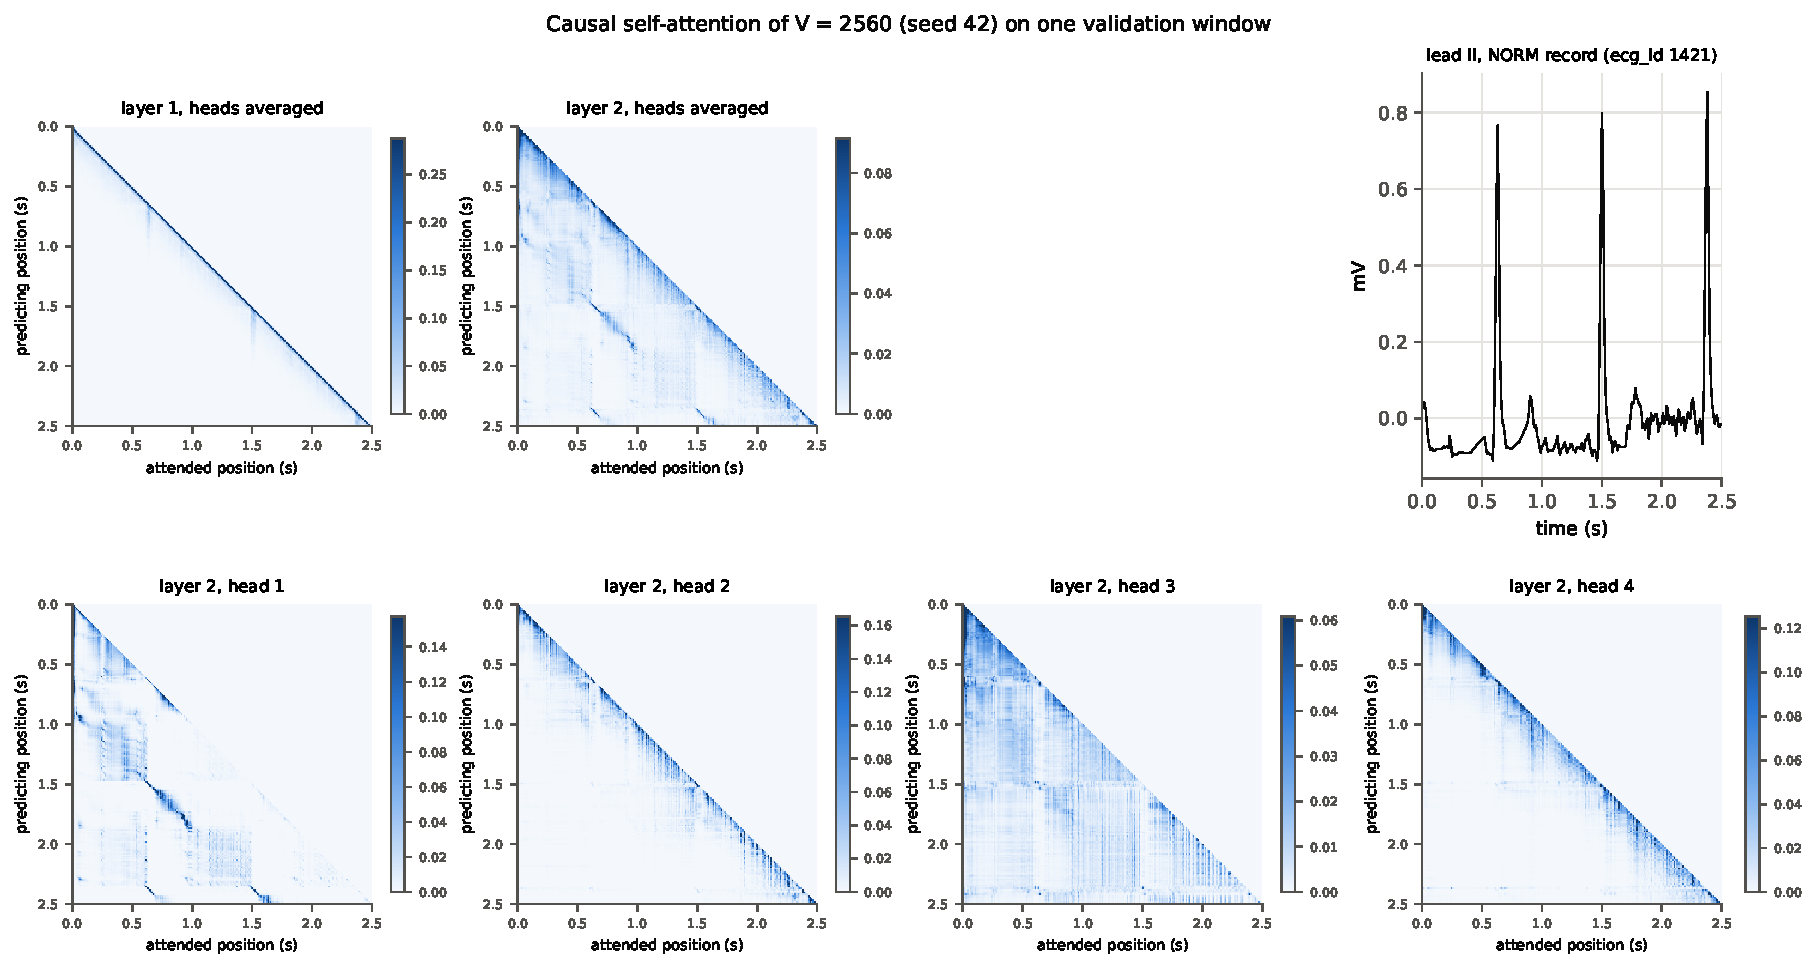
\includegraphics[width=\textwidth,height=0.42\textheight,keepaspectratio]{figures/generative_attention.pdf}
\caption[ECG-GPT: causal self-attention maps]{Causal self-attention of the selected ECG-GPT ($V = 2560$, seed 42) on one validation window of 2.5\,s (NORM record, right): both layers with the heads averaged and the four heads of layer 2. Row: predicting position; column: attended position; everything above the diagonal is zero.}
\label{fig:generative_attention}
\end{figure}


\paragraph{Caveats.} The heart rate comes from a simple threshold rule on R peaks, not a validated
detector. The cross-entropy at the last position of a window also mixes in an effect of the end of the
record (the cost rises sharply there for every model); this is a hypothesis we did not test directly,
and it only affects comparisons of that column across context lengths. Nothing was generated without a
prompt.
